% ============================================================
% F1 CHAMPIONSHIP MANAGEMENT SYSTEM — BÁO CÁO DBMS
% Biên dịch trên Overleaf: pdfLaTeX
% ============================================================
\documentclass[12pt, a4paper]{report}

% --- Encoding ---
\usepackage[utf8]{inputenc}
\usepackage[T5]{fontenc}
\usepackage[english]{babel}

% --- Font Times New Roman equivalent ---
\usepackage{mathptmx}

% --- Page layout (Tuân thủ yêu cầu: Phải 3cm, Trái/Trên/Dưới 2cm) ---
\usepackage[
  a4paper,
  top=2cm,
  bottom=2cm,
  left=2cm,
  right=3cm
]{geometry}

%---- bìa
\usepackage{tikz}
\usetikzlibrary{calc}

% --- Line spacing (Dãn dòng đơn) ---
\usepackage{setspace}
\singlespacing

% --- Headers & Footers ---
\usepackage{fancyhdr}
\pagestyle{fancy}
\fancyhf{}
\fancyhead[L]{\small\textit{F1 Championship Management System}}
\fancyhead[R]{\small\textit{DBMS Report}}
\fancyfoot[C]{\thepage}
\renewcommand{\headrulewidth}{0.4pt}

% --- Colors ---
\usepackage{xcolor}
\definecolor{codeblue}{RGB}{0,82,162}
\definecolor{codegray}{RGB}{245,245,245}
\definecolor{codecomment}{RGB}{90,120,90}
\definecolor{codestring}{RGB}{163,21,21}
\definecolor{codekw}{RGB}{0,0,200}
\definecolor{tableheadbg}{RGB}{31,73,125}
\definecolor{tableheadfg}{RGB}{255,255,255}
\definecolor{rowalt}{RGB}{235,241,250}
\definecolor{f1red}{RGB}{225,6,0}

% --- Tables ---
\usepackage{booktabs}
\usepackage{tabularx}
\usepackage{longtable}
\usepackage{colortbl}
\usepackage{multirow}
\usepackage{array}
\newcolumntype{L}[1]{>{\raggedright\arraybackslash}p{#1}}
\newcolumntype{C}[1]{>{\centering\arraybackslash}p{#1}}

%------
\usepackage[table]{xcolor} % Quan trọng để dùng màu cho bảng
\usepackage{tabularx}
\usepackage{caption}
\usepackage[most]{tcolorbox} % Gói lệnh quan trọng để bo góc và tạo viền

% --- Code listings ---
\usepackage{listings}
\lstdefinestyle{sqlstyle}{
  language=SQL,
  basicstyle=\ttfamily\small,
  backgroundcolor=\color{codegray},
  keywordstyle=\color{codekw}\bfseries,
  stringstyle=\color{codestring},
  commentstyle=\color{codecomment}\itshape,
  morecomment=[l]{--},
  morestring=[b]',
  morestring=[b]",
  breaklines=true,
  breakatwhitespace=false,
  numbers=left,
  numberstyle=\tiny\color{gray},
  numbersep=8pt,
  frame=single,
  framerule=0.4pt,
  rulecolor=\color{gray!50},
  showstringspaces=false,
  tabsize=4,
  captionpos=b,
  xleftmargin=15pt,
  morekeywords={DELIMITER, SIGNAL, SQLSTATE, MESSAGE_TEXT, RANK, OVER,
                PARTITION, TIMESTAMPDIFF, MICROSECOND, RESIGNAL,
                PROCEDURE, FUNCTION, BEGIN, DECLARE, INTO, HANDLER,
                SQLEXCEPTION, AUTO_INCREMENT, TINYINT, DATETIME, ENUM,
                DEFAULT, CONSTRAINT, CHECK, VIEW, TRIGGER, BEFORE,
                EACH, ROW, CALL, START, TRANSACTION, ROLLBACK, COMMIT}
}
\lstset{style=sqlstyle}

% --- Flowchart / Diagram ---
\usepackage{tikz}
\usetikzlibrary{shapes.geometric, arrows.meta, positioning, fit, backgrounds}
\tikzstyle{process}=[rectangle, rounded corners=4pt, minimum width=7cm,
  minimum height=0.9cm, text centered, draw=codeblue, fill=blue!8, font=\small]
\tikzstyle{arrow}=[-{Stealth[length=6pt]}, thick, color=codeblue]
\tikzstyle{decision}=[diamond, aspect=3, minimum width=4cm,
  draw=f1red, fill=red!8, font=\small\bfseries]

% --- Hyperlinks ---
\usepackage{hyperref}
\hypersetup{
  colorlinks=true,
  linkcolor=black,
  urlcolor=codeblue,
  pdfauthor={Group 6},
  pdftitle={DBMS Report - F1 Championship Management System}
}

% --- Graphics ---
\usepackage{graphicx}
\usepackage{float}

% --- Miscellaneous ---
\usepackage{enumitem}
\usepackage{amsmath}
\usepackage{amssymb}
\usepackage{caption}
\usepackage{subcaption}
\usepackage{titlesec}
\usepackage{tocloft}
\usepackage{mdframed}
\usepackage[most]{tcolorbox}
\usepackage{indentfirst}

% --- Formatting titles ---
\titleformat{\chapter}[display]
  {\normalfont\Huge\bfseries\color{black}}{\chaptertitlename\ \thechapter}{20pt}{\Huge}
\titlespacing*{\chapter}{0pt}{-20pt}{20pt}

% ============================================================
\usepackage{xcolor}
\usepackage[most]{tcolorbox}
\newtcolorbox{note_box}{
  colback=green!5,          % Màu nền xanh nhạt (giống ảnh)
  colframe=green!30!black,  % Màu viền và thanh header (xanh đậm)
  coltitle=white,           % Màu chữ tiêu đề (trắng)
  fonttitle=\bfseries\small,% Kiểu chữ tiêu đề (đậm, nhỏ)
  title=NOTE,               % Nội dung thanh header
  sharp corners,            % Góc vuông giống cái bảng trong ảnh
  enhanced,
  boxrule=0.5pt,            % Độ dày viền
  left=10pt, right=10pt,    % Khoảng cách lề trong khung
  top=5pt, bottom=5pt
}
\definecolor{darkblue}{RGB}{31, 73, 125}     % Màu xanh đậm cho tiêu đề chính
\definecolor{mediumblue}{RGB}{52, 101, 164} % Màu cho tiêu đề cột
\definecolor{lightblue}{RGB}{235, 241, 250}
\begin{document}
% ============================================================

% ---- COVER PAGE ----
\begin{titlepage}
    \begin{tikzpicture}[remember picture, overlay]
        % Khung ngoài rất đậm (line width = 5pt hoặc 6pt)
        \draw[line width = 5pt] (current page.north west) rectangle (current page.south east);
        
        % Khung phụ bên trong cũng đậm hơn một chút (line width = 1.5pt hoặc 2pt)
        % Tăng khoảng cách cách mép lên một chút (3mm) để hai đường không bị dính vào nhau khi đường ngoài quá dày
        \draw[line width = 1.5pt] ($(current page.north west) + (3mm,-3mm)$) rectangle ($(current page.south east) + (-3mm,3mm)$);
    \end{tikzpicture}

    \centering
    
    {\large \textbf{POSTS AND TELECOMMUNICATIONS INSTITUTE OF TECHNOLOGY}} \\
    {\large \textbf{FACULTY OF INFORMATION TECHNOLOGY}} \\
    \vspace{0.5cm}
    {\large \textbf{DATABASE MANAGEMENT SYSTEMS}} \\
    
    \vspace{1cm}
    % Chèn logo vào đây. Thay 'logo-ptit.png' bằng tên file ảnh của bạn
    \includegraphics[width=7cm]{logo.png} 
    
    \vspace{2.5cm}
    
    {\large \textbf{GROUP PROJECT REPORT - GROUP 6}} \\
    \vspace{0.5cm}
    {\Large \textbf{F1 CHAMPIONSHIP MANAGEMENT SYSTEM}} \\
    
    \vfill
    
    \begin{flushleft}
    \hspace{0.5cm}
    {\Large % Bắt đầu cụm chữ lớn hơn cho phần thông tin
    \renewcommand{\arraystretch}{1.2} % Giãn dòng trong bảng cho thoáng
    \begin{tabular}{ll}
        \textbf{Supervisor:} & Assoc. Prof. Dr. Nguyen Trong Khanh \\
        \textbf{Team members:} & Nguyen Van Hieu - B23DCCE033 \\
        & Pham Nhat Minh - B23DCCE066 \\
        & Le Minh Duc - B23DCVT095 \\
    \end{tabular}
    }
    \end{flushleft}
    
    \vspace{2.5cm}
    
    {\large Hanoi, April 2026}

\end{titlepage}
% ---- TABLE OF CONTENTS ----
\cleardoublepage 
\pagenumbering{arabic}
\tableofcontents
\newpage

\listoffigures 
\newpage

\listoftables 
\newpage

\lstlistoflistings 
\newpage

% --- Định nghĩa bảng màu theo ảnh mẫu ---
\definecolor{headergreen}{RGB}{0, 128, 0}       % Xanh lá đậm (Tiêu đề chính)
\definecolor{rowgreen}{RGB}{235, 250, 235}     % Xanh lá rất nhạt (Dòng xen kẽ)
\definecolor{textgreen}{RGB}{0, 100, 0}        % Chữ xanh đậm cho tiêu đề cột

\begin{center}
    % Cấu hình khung bên ngoài (tcolorbox)
    \begin{tcolorbox}[
        enhanced,
        arc=10pt,            % Độ bo góc
        outer arc=10pt,
        boxrule=1.5pt,       % Độ dày viền
        colframe=headergreen, % Màu viền
        colback=white,       % Màu nền trong
        clip upper,          % Cắt nội dung thừa ở góc bo
        left=0pt, right=0pt, top=0pt, bottom=0pt, % Sát lề khung
        boxsep=0pt,
        fonttitle=\bfseries\large,
        colbacktitle=headergreen,
        title={Database Terminology Glossary},
        halign title=center,
        toptitle=3mm, bottomtitle=3mm
    ]
        
        % Nội dung bảng bên trong
        \renewcommand{\arraystretch}{1.6}
        \rowcolors{2}{rowgreen}{white} % Đổ màu từ dòng đầu tiên của bảng (sau tiêu đề tcolorbox)
        
        \begin{tabularx}{\textwidth}{>{\hspace{1em}\bfseries\color{textgreen}}l X<{\hspace{1em}}}
            % Tiêu đề cột
            \rowcolor{white}
            \textcolor{textgreen}{\textbf{Term}} & \textcolor{textgreen}{\textbf{Definition}} \\
            \hline
            
            % Dữ liệu
            ACID & A set of four properties (Atomicity, Consistency, Isolation, Durability) that guarantee the reliability of database transactions. \\
        
            MVCC & (Multi-Version Concurrency Control) A mechanism that supports concurrent access by allowing multiple versions of data to exist simultaneously. \\
            
            DBA & (Database Administrator) The administrator responsible for operating, securing, and optimizing the database system. \\
            
            InnoDB engine & The default storage engine for MySQL that supports ACID transactions, row-level locking, and crash recovery features. \\
            
            B+ Tree & A self-balancing tree data structure that optimizes search and block-based data retrieval in DBMS. \\
            
            Buffer pool & A RAM memory area used to cache data and indexes, minimizing direct disk read/write operations. \\
            
            Redo log & A log that records data changes to restore system state in the event of an unexpected failure. \\
            
            Undo log & A log that records the previous state of data to support rollback operations and the MVCC mechanism. \\
            
            Trigger & A SQL code object that automatically executes when an INSERT, UPDATE, or DELETE event occurs on a table. \\
            
            Transaction & A logical unit of work consisting of a sequence of SQL operations, ensuring either complete execution or no execution at all. \\
            
            Stored Procedure & A set of precompiled SQL statements stored on the server to execute recurring business operations. \\
            
            Views & A virtual table that presents data from one or more tables through a predefined query statement. \\
            
            Index & A data structure that speeds up record lookup, similar to the index of a book. \\
            
            JWT Authentication & (JSON Web Token) A secure authentication method between system components using encoded tokens. \\
            
            CTE & (Common Table Expression) A temporary result set that makes complex SQL statements clearer and easier to manage. \\
            \hline
        \end{tabularx}
    \end{tcolorbox}
\end{center}

% ============================================================
\chapter{Problem Introduction}
% ============================================================

\section{Context}
Formula 1 (F1) is the world's premier open-wheel racing championship. With dozens of teams, over 20 professional drivers, and a race calendar spanning nearly an entire year, managing the data lifecycle of this global sport demands precision and high data integrity. Each season comprises multiple races (Grand Prix) held across different countries.

\textbf{The F1 Championship Management System} is a comprehensive software platform designed to manage data across multiple seasons. Before having a centralized DBMS, managing driver contracts, team assignments, lap completion times, and scoring was highly error-prone. This system leverages the Relational Database Management System (RDBMS) model to provide a centralized, consistent, and highly available data repository.

\section{System Objectives}
The system is built to automate the core operations of an F1 season, specifically:
\begin{itemize}[leftmargin=1.5cm]
    \item Manage information about teams, drivers, and their active contracts.
    \item Schedule races and manage Grand Prix events across seasons.
    \item Register drivers for specific races based on strict business rules.
    \item Record race results in real-time and automatically calculate points according to the international FIA standard.
    \item Provide accurate and continuously updated driver and constructor standings.
\end{itemize}

\section{Functional Requirements (FR)}
The system must fulfill the following functional requirements:
\begin{description}[leftmargin=1.5cm, style=nextline]
    \item[FR-01] Manage F1 season information (Create, Update, Read).
    \item[FR-02] Manage the list of teams and drivers, including contract history.
    \item[FR-03] Allow driver registration for each race, with a constraint of a maximum of 2 drivers per team per race.
    \item[FR-04] Allow entry of race results (finish time, laps completed, status).
    \item[FR-05] Automatically calculate points according to the F1 standard (P1=25, P2=18, P3=15, etc.) immediately after saving results.
    \item[FR-06] Provide driver and constructor standings, with filtering support by race history.
    \item[FR-07] Support race result adjustments after saving, with automatic score recalculation.
\end{description}

\section{Core Business Rules}
The database logic is designed to strictly enforce the following rules:
\begin{enumerate}
    \item \textbf{Driver limit:} A team is not allowed to register more than two drivers in the same race.
    \item \textbf{Scoring system:} Points are calculated based on time ranking. Only drivers who finish the race (\texttt{status = 'Finished'}) are eligible for points.
    \item \textbf{Time validity:} The finish time (\texttt{end\_time}) must be greater than the race start time.
    \item \textbf{Contract management:} When a driver transfers to another team, the old contract is set to \texttt{is\_active = 0}, and a new contract is created with \texttt{is\_active = 1}.
    \item \textbf{Constructor points:} The total points of a team at a race equals the sum of points of all drivers belonging to that team at the race.
\end{enumerate}

% ============================================================
\chapter{Configuration, Tools, and Platform}
% ============================================================

During the development of the F1 Championship Management System, the selection of hardware, platform technologies, and software architecture plays a decisive role in the system's performance, data integrity, and scalability. Below is a detailed analysis of the environment and tools used by the team.

\section{Hardware Environment and Deployment Configuration}

The system was developed, tested, and load-tested on a personal computer serving as a local server. The hardware configuration not only supports running the source code but must also meet the demanding I/O requirements of the DBMS.

\begin{table}[h]
\centering
\caption{Hardware configuration of the development environment}
\begin{tabularx}{\textwidth}{L{4cm} L{11.2cm}}
\toprule
\rowcolor{tableheadbg}
\textcolor{white}{\textbf{Component}} & \textcolor{white}{\textbf{Details and Rationale}} \\
\midrule
Operating System & Windows 11 Pro 64-bit / Linux Ubuntu 22.04 LTS. Provides a stable environment for running MySQL and Node.js background services. \\
\rowcolor{rowalt}
Processor (CPU) & Intel Core i5 12th Gen or equivalent. Ensures smooth processing of complex queries containing Window Functions and Subqueries. \\
Memory (RAM) & 8 GB - 16 GB DDR4. \textbf{Significance for DBMS:} Provides sufficient capacity for the InnoDB Buffer Pool, enabling data and index caching in RAM, minimizing disk I/O. \\
\rowcolor{rowalt}
Storage & 256 GB SSD (NVMe preferred). \textbf{Significance for DBMS:} The high random write speed of SSDs is crucial for fast Redo Log and Undo Log writes, ensuring Transaction Durability. \\
\bottomrule
\end{tabularx}
\end{table}

\clearpage
\section{Technologies Used}
The application uses a modern technology stack, clearly separated via the 3-Tier Architecture model.

\begin{table}[h]
\centering
\caption{Technology and platform overview}
\begin{tabularx}{\textwidth}{L{2.5cm} L{4.5cm} L{2.5cm} L{4.8cm}}
\toprule
\rowcolor{tableheadbg}
\textcolor{white}{\textbf{Tier}} & \textcolor{white}{\textbf{Technology}} & \textcolor{white}{\textbf{Version}} & \textcolor{white}{\textbf{Role}} \\
\midrule
Database    & MySQL / MariaDB         & 8.0 / 10.6+ & Relational DBMS \\
\rowcolor{rowalt}
Backend     & Node.js                 & 18.x LTS    & JavaScript runtime environment \\
Backend     & Express.js              & 4.x         & RESTful API framework \\
\rowcolor{rowalt}
DB Driver   & mysql2/promise          & 3.x         & Async Node.js-MySQL connector \\
Frontend    & React.js (Vite)         & 18.x        & SPA UI rendering library \\
\rowcolor{rowalt}
Frontend    & TailwindCSS             & 3.x         & Utility-first CSS framework \\
DB Admin    & MySQL Workbench         & 8.x         & DB design and query tool \\
\bottomrule
\end{tabularx}
\end{table}

\section{Architecture Rationale}
The system is designed following the \textbf{3-Tier Architecture}:

\begin{enumerate}
    \item \textbf{Presentation Tier (React.js):} Provides a smooth Single Page Application (SPA) experience. Vite is used to leverage extremely fast build speeds (HMR).
    \item \textbf{Application Tier (Node.js/Express.js):} Acts as middleware for processing logic. Using JavaScript for both Frontend and Backend reduces context-switching costs. The \texttt{mysql2} library was chosen for its Promise API support, enabling safe \texttt{async/await} usage and efficient connection pool management.
    \item \textbf{Data Tier (MySQL/InnoDB):} MySQL was chosen for its excellent support for the relational model, ACID transactions, Stored Procedures, and Triggers. The InnoDB engine plays a critical role with its row-level locking mechanism, preventing bottlenecks when multiple threads update race results simultaneously.
\end{enumerate}

% ============================================================
\chapter{Installation \& Deployment}
% ============================================================

This chapter describes in detail the database design process, SQL scripts (DDL, Triggers, Procedures, Views), and deployment steps.

\section{Database Design and Normalization}

The database schema was rigorously designed to achieve \textbf{BCNF (Boyce-Codd Normal Form)}, ensuring data integrity and completely eliminating redundancy.


\subsection{Relational Schema}
\begin{itemize}
    \item \texttt{CHAMPIONSHIPS(\underline{champ\_code}, name, description)}
    \item \texttt{TEAMS(\underline{team\_code}, name, brand, owner, description)}
    \item \texttt{DRIVERS(\underline{driver\_code}, name, date\_of\_birth, nationality)}
    \item \texttt{CONTRACTS(\underline{contract\_id}, driver\_code*, team\_code*, is\_active)}
    \item \texttt{RACES(\underline{race\_code}, name, num\_laps, start\_time, champ\_code*)}
    \item \texttt{RACE\_ENTRIES(\underline{entry\_id}, race\_code*, contract\_id*)}
    \item \texttt{RESULTS(\underline{entry\_id*}, end\_time, laps\_completed, status, points)}
    \item \texttt{SPONSORS(\underline{sponsor\_code}, name, industry, description)}
    \item \texttt{TEAM\_SPONSORSHIPS(\underline{sponsorship\_id}, team\_code*, sponsor\_code*, funding\_amount, start\_year, end\_year)}
    \item \texttt{PENALTIES(\underline{penalty\_id}, entry\_id*, type, severity\_value, reason, is\_applied)}
\end{itemize}
\textit{(* denotes Foreign Key)}

\begin{tcolorbox}[
    enhanced, breakable,    % Giúp khung tự ngắt trang nếu danh sách quá dài
    colback=blue!5,         % Màu nền xanh rất nhẹ
    colframe=blue!50!black, % Màu viền xanh đậm
    boxrule=0.5pt,          % Độ dày viền mảnh
    arc=2pt,                % Bo góc nhẹ
    left=10pt, right=10pt,  % Khoảng cách lề trái/phải bên trong khung
    top=8pt, bottom=8pt     % Khoảng cách lề trên/dưới bên trong khung
]
{\large \textit{Detailed Explanation:}} \\ [12pt]


The system consists of 10 main entities (tables), designed to comprehensively manage the lifecycle of an F1 racing season.

\begin{itemize}[leftmargin=1.5cm]
    \item \textbf{CHAMPIONSHIPS (Seasons):} Stores information about racing seasons.
    \begin{itemize}
        \item \textit{Attributes:} \texttt{\underline{champ\_code}} (VARCHAR(10) - Season code - PK), \texttt{name} (VARCHAR(255) - Season name), \texttt{description} (TEXT - Description).
    \end{itemize}

    \item \textbf{TEAMS (Racing Teams):} Manages information about participating teams.
    \begin{itemize}
        \item \textit{Attributes:} \texttt{\underline{team\_code}} (VARCHAR(10) - Team code - PK), \texttt{name} (VARCHAR(100) - Team name), \texttt{brand} (VARCHAR(100) - Car brand), \texttt{owner} (VARCHAR(100) - Owner), \texttt{description} (TEXT - Description).
    \end{itemize}

    \item \textbf{DRIVERS (Drivers):} Manages driver profile information.
    \begin{itemize}
        \item \textit{Attributes:} \texttt{\underline{driver\_code}} (VARCHAR(10) - Driver code - PK), \texttt{name} (VARCHAR(100) - Name), \texttt{date\_of\_birth} (DATE - Date of birth), \texttt{nationality} (VARCHAR(50) - Nationality), \texttt{biography} (TEXT - Biography).
    \end{itemize}

    \item \textbf{CONTRACTS (Contracts):} Junction table storing the signing history between Drivers and Teams.
    \begin{itemize}
        \item \textit{Attributes:} \texttt{\underline{contract\_id}} (INT - Contract ID - PK), \texttt{driver\_code} (VARCHAR(10) - Driver code - FK), \texttt{team\_code} (VARCHAR(10) - Team code - FK), \texttt{is\_active} (TINYINT - Active status).
    \end{itemize}

    \item \textbf{RACES (Races):} Information about each race in a season.
    \begin{itemize}
        \item \textit{Attributes:} \texttt{\underline{race\_code}} (VARCHAR(10) - Race code - PK), \texttt{name} (VARCHAR(100) - Race name), \texttt{num\_laps} (INT - Number of laps), \texttt{location} (VARCHAR(255) - Location), \texttt{start\_time} (DATETIME(3) - Start time), \texttt{champ\_code} (VARCHAR(10) - Season code - FK), \texttt{description} (TEXT - Description).
    \end{itemize}

    \item \textbf{RACE\_ENTRIES (Race Entries):} Junction table recording driver registration (via contract) for a specific race.
    \begin{itemize}
        \item \textit{Attributes:} \texttt{\underline{entry\_id}} (INT - Entry ID - PK), \texttt{race\_code} (VARCHAR(10) - Race code - FK), \texttt{contract\_id} (INT - Contract ID - FK).
    \end{itemize}

    \item \textbf{RESULTS (Race Results):} Records driver performance after a race.
    \begin{itemize}
        \item \textit{Attributes:} \texttt{\underline{entry\_id}} (INT - Entry ID - PK/FK), \texttt{end\_time} (DATETIME(3) - Finish time), \texttt{laps\_completed} (INT - Laps completed), \texttt{status} (ENUM - Status Finished/DNF/Accident), \texttt{points} (INT - Points).
    \end{itemize}

    \item \textbf{SPONSORS (Sponsors):} Manages list of sponsors.
    \begin{itemize}
        \item \textit{Attributes:} \texttt{\underline{sponsor\_code}} (VARCHAR(10) - Sponsor code - PK), \texttt{name} (VARCHAR(100) - Sponsor name), \texttt{industry} (VARCHAR(50) - Industry), \texttt{description} (TEXT - Description).
    \end{itemize}

    \item \textbf{TEAM\_SPONSORSHIPS (Team Sponsorships):} Junction table tracking funding history between sponsors and teams.
    \begin{itemize}
        \item \textit{Attributes:} \texttt{\underline{sponsorship\_id}} (INT - Sponsorship ID - PK), \texttt{team\_code} (VARCHAR(10) - Team code - FK), \texttt{sponsor\_code} (VARCHAR(10) - Sponsor code - FK), \texttt{funding\_amount} (DECIMAL(15,2) - Funding amount), \texttt{start\_year} (INT - Start year), \texttt{end\_year} (INT - End year).
    \end{itemize}

    \item \textbf{PENALTIES (Penalties):} Records driver penalties during races.
    \begin{itemize}
        \item \textit{Attributes:} \texttt{\underline{penalty\_id}} (INT - Penalty ID - PK), \texttt{entry\_id} (INT - Entry ID - FK), \texttt{type} (VARCHAR(50) - Penalty type), \texttt{severity\_value} (INT - Penalty severity value), \texttt{reason} (VARCHAR(255) - Reason), \texttt{is\_applied} (TINYINT - Applied status).
    \end{itemize}
\end{itemize}
\end{tcolorbox}

Based on the foreign key structure, the entities in the system have the following relationships:

\begin{enumerate}[leftmargin=1.5cm]
    \item \textbf{Championship - Race (1:N):} A championship (\texttt{CHAMPIONSHIPS}) includes multiple races (\texttt{RACES}).
    \item \textbf{Team - Contract (1:N):} A team (\texttt{TEAMS}) can sign multiple contracts (\texttt{CONTRACTS}) with different drivers.
    \item \textbf{Driver - Contract (1:N):} A driver (\texttt{DRIVERS}) can have multiple contracts (\texttt{CONTRACTS}) with different teams throughout their career.
    \item \textbf{Race - Entry (1:N):} Each race (\texttt{RACES}) has multiple race entries (\texttt{RACE\_ENTRIES}).
    \item \textbf{Contract - Entry (1:N):} A contract (\texttt{CONTRACTS} - representing 1 driver of 1 team) can be used to register for multiple races (\texttt{RACE\_ENTRIES}).
    \item \textbf{Entry - Result (1:1):} Each race entry (\texttt{RACE\_ENTRIES}) has exactly one corresponding result record (\texttt{RESULTS}).
    \item \textbf{Team - Sponsor (N:M):} Sponsors (\texttt{SPONSORS}) can sponsor multiple teams, and teams (\texttt{TEAMS}) can be sponsored by multiple sponsors, managed via \texttt{TEAM\_SPONSORSHIPS}.
    \item \textbf{Entry - Penalty (1:N):} A race entry (\texttt{RACE\_ENTRIES}) can receive multiple penalties (\texttt{PENALTIES}).
\end{enumerate}

\begin{figure}[H]
    \centering
    % Thay 'kientruc.png' bằng tên file ảnh thực tế bạn đã tải lên
    % width=0.8\textwidth nghĩa là ảnh sẽ rộng bằng 80% chiều rộng trang giấy
    \includegraphics[width=0.8\textwidth]{DB.png} 
    \caption{Entity-Relationship Diagram (ERD)}
    \label{fig:kientruc}
\end{figure}


\subsection{Normalization Assessment}
\begin{itemize}
    \item \textbf{First Normal Form (1NF):} All attributes are atomic. There are no repeating groups. For example: a team's driver list is managed through multiple records in \texttt{CONTRACTS} rather than using a comma-separated text string.
    \item \textbf{Second Normal Form (2NF):} All tables satisfy 1NF and have no partial dependencies. The \texttt{RACE\_ENTRIES} table uses a surrogate key (\texttt{entry\_id}) instead of a composite key, completely eliminating the possibility of 2NF violations.
    \item \textbf{Third Normal Form (3NF) \& BCNF:} The schema eliminates all transitive dependencies. For instance, \texttt{team\_name} does not appear in \texttt{RACE\_ENTRIES}. Every determinant in the system is a superkey.
\end{itemize}

\section{Data Definition Language (DDL) Script}

The following SQL code initializes the database, table structures, and establishes foreign keys.

\begin{lstlisting}[caption={DDL --- Table creation and constraint setup}]
DROP DATABASE IF EXISTS F1_Championship_Management;
CREATE DATABASE F1_Championship_Management;
USE F1_Championship_Management;

SET SQL_SAFE_UPDATES = 0;

CREATE TABLE CHAMPIONSHIPS (
    champ_code  VARCHAR(10)  PRIMARY KEY,
    name        VARCHAR(255) NOT NULL,
    description TEXT
);

CREATE TABLE TEAMS (
    team_code   VARCHAR(10)  PRIMARY KEY,
    name        VARCHAR(100) NOT NULL,
    brand       VARCHAR(100),
    owner       VARCHAR(100),
    description TEXT
);

CREATE TABLE DRIVERS (
    driver_code   VARCHAR(10)  PRIMARY KEY,
    name          VARCHAR(100) NOT NULL,
    date_of_birth DATE,
    nationality   VARCHAR(50),
    biography     TEXT
);

CREATE TABLE CONTRACTS (
    contract_id INT          AUTO_INCREMENT PRIMARY KEY,
    driver_code VARCHAR(10),
    team_code   VARCHAR(10),
    is_active   TINYINT      DEFAULT 1,
    FOREIGN KEY (driver_code) REFERENCES DRIVERS(driver_code),
    FOREIGN KEY (team_code)   REFERENCES TEAMS(team_code)
);

CREATE TABLE RACES (
    race_code   VARCHAR(10)  PRIMARY KEY,
    name        VARCHAR(100) NOT NULL,
    num_laps    INT          NOT NULL,
    location    VARCHAR(255),
    start_time  DATETIME(3),
    champ_code  VARCHAR(10),
    description TEXT,
    FOREIGN KEY (champ_code) REFERENCES CHAMPIONSHIPS(champ_code)
);

CREATE TABLE RACE_ENTRIES (
    entry_id    INT AUTO_INCREMENT PRIMARY KEY,
    race_code   VARCHAR(10),
    contract_id INT,
    FOREIGN KEY (race_code)   REFERENCES RACES(race_code),
    FOREIGN KEY (contract_id) REFERENCES CONTRACTS(contract_id),
    UNIQUE(race_code, contract_id)
);

CREATE TABLE RESULTS (
    entry_id       INT PRIMARY KEY,
    end_time       DATETIME(3),
    laps_completed INT,
    status         ENUM('Finished', 'DNF', 'Accident') DEFAULT 'Finished',
    points         INT DEFAULT 0,
    FOREIGN KEY (entry_id) REFERENCES RACE_ENTRIES(entry_id),
    CONSTRAINT chk_laps_completed CHECK (laps_completed >= 0),
    CONSTRAINT chk_points         CHECK (points >= 0)
);
\end{lstlisting}

\section{Database Triggers for Business Logic}
Embedding business logic at the database layer ensures that rules cannot be bypassed, regardless of whether data is entered via the API or directly through a DB admin tool.

\subsection{Limiting the Number of Drivers per Team}

\textbf{Purpose:} Prevent the registration of a 3rd driver from the same team in the same race.


\begin{figure}[h]
\centering
\hspace*{-1.5cm} % <--- Lệnh kéo hình lệch sang trái (có thể tăng/giảm số -1.5)
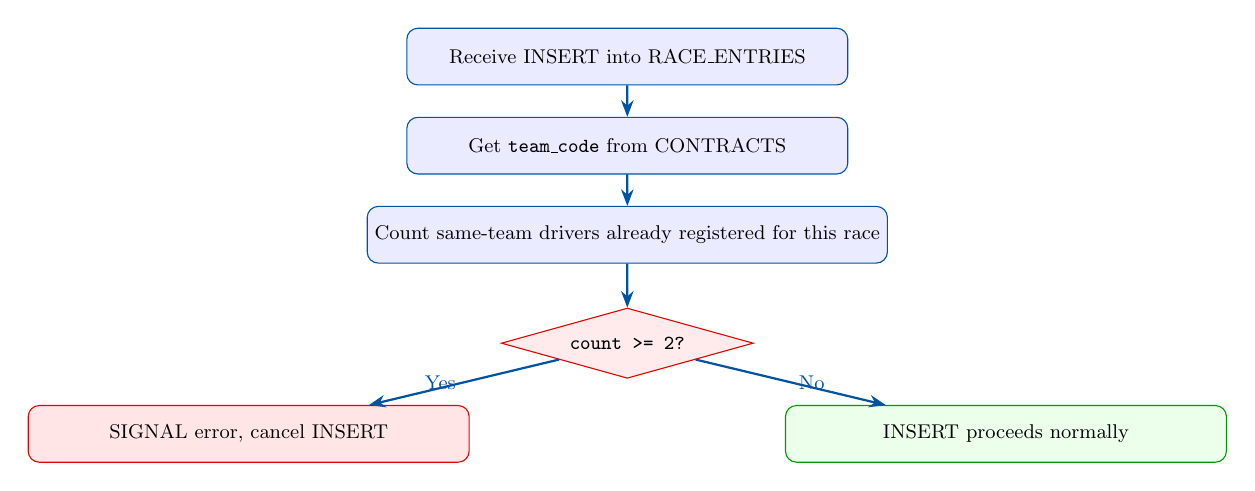
\begin{tikzpicture}[node distance=0.5cm, scale=0.8, transform shape] % <--- Thêm scale=0.8 để thu nhỏ hình
  \node[process] (a) {Receive INSERT into RACE\_ENTRIES};
  \node[process, below=of a] (b) {Get \texttt{team\_code} from CONTRACTS};
  \node[process, below=of b] (c) {Count same-team drivers already registered for this race};
  \node[decision, below=0.7cm of c] (d) {\texttt{count >= 2?}};
  \node[process, below left=0.7cm and 1.5cm of d, fill=red!10, draw=f1red]
    (e) {SIGNAL error, cancel INSERT};
  \node[process, below right=0.7cm and 1.5cm of d, fill=green!8, draw=green!60!black]
    (f) {INSERT proceeds normally};
  \draw[arrow] (a)--(b);
  \draw[arrow] (b)--(c);
  \draw[arrow] (c)--(d);
  \draw[arrow] (d) -- node[left,font=\small]{Yes} (e);
  \draw[arrow] (d) -- node[right,font=\small]{No} (f);
\end{tikzpicture}
\caption{Processing flow of Trigger trg\_limit\_2\_riders}
\end{figure}

This trigger ensures no team registers more than 2 drivers in the same race.
\begin{lstlisting}[caption={Trigger --- trg\_limit\_2\_riders}]
DELIMITER //
CREATE TRIGGER trg_limit_2_riders
BEFORE INSERT ON RACE_ENTRIES
FOR EACH ROW
BEGIN
    DECLARE v_team_id VARCHAR(10);
    DECLARE v_count INT;
    
    -- Lay ma doi cua tay dua sap dang ky
    SELECT team_code INTO v_team_id 
    FROM CONTRACTS WHERE contract_id = NEW.contract_id;
    
    -- Dem so tay dua cua doi nay da dang ky trong chang
    SELECT COUNT(*) INTO v_count 
    FROM RACE_ENTRIES re 
    JOIN CONTRACTS c ON re.contract_id = c.contract_id
    WHERE re.race_code = NEW.race_code 
      AND c.team_code = v_team_id;
      
    -- Huy giao dich neu vuot qua so luong cho phep
    IF v_count >= 2 THEN
        SIGNAL SQLSTATE '45000' 
        SET MESSAGE_TEXT = 'Error: Each team can register a maximum of 2 drivers!';
    END IF;
END //
DELIMITER ;
\end{lstlisting}

\subsection{Time Validity Check}
\textbf{Purpose:} Ensure \texttt{end\_time > start\_time} of the race. Applied to both INSERT and UPDATE on the RESULTS table.
This trigger ensures the finish time occurs after the race start time.
\begin{lstlisting}[caption={Trigger --- trg\_check\_time\_insert}]
DELIMITER //
CREATE TRIGGER trg_check_time_insert
BEFORE INSERT ON RESULTS
FOR EACH ROW
BEGIN
    DECLARE v_start_time DATETIME(3);
    IF NEW.status = 'Finished' AND NEW.end_time IS NOT NULL THEN
        SELECT r.start_time INTO v_start_time 
        FROM RACE_ENTRIES re 
        JOIN RACES r ON re.race_code = r.race_code 
        WHERE re.entry_id = NEW.entry_id;
        
        IF NEW.end_time <= v_start_time THEN
            SIGNAL SQLSTATE '45000' 
            SET MESSAGE_TEXT = 
              'Error: Finish time must be greater than start time!';
        END IF;
    END IF;
END //
DELIMITER ;
\end{lstlisting}
\textbf{Rationale for database-level constraints:} If validation is only performed at the Frontend or Backend, users can bypass it using Postman or MySQL Workbench. Triggers ensure constraints are enforced at \textbf{EVERY ACCESS POINT}.

\section{Stored Procedure and Transaction}
\textbf{Purpose:} Automatically calculate F1 points based on time ranking, wrapped in an ACID Transaction.

F1 point calculation requires ranking drivers by their finish times. Performing this dynamically via a View would degrade performance. Therefore, a Stored Procedure is called immediately after saving results. This process runs inside a Transaction to ensure Atomicity.
 \newpage
\begin{figure}[h]
\centering
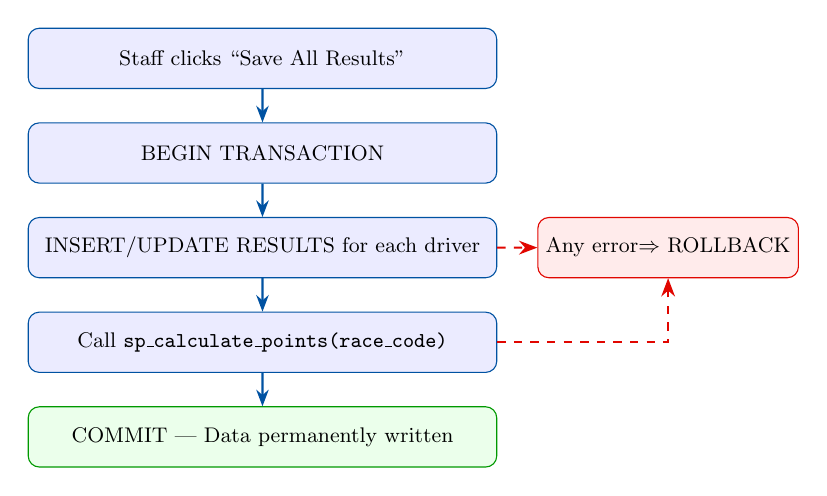
\begin{tikzpicture}[node distance=0.5cm, scale=0.85, transform shape]
  \node[process] (t1) {Staff clicks ``Save All Results''};
  \node[process, below=of t1] (t2) {BEGIN TRANSACTION};
  \node[process, below=of t2] (t3) {INSERT/UPDATE RESULTS for each driver};
  \node[process, below=of t3] (t4) {Call \texttt{sp\_calculate\_points(race\_code)}};
  \node[process, below=of t4, fill=green!8, draw=green!60!black]
    (t5) {COMMIT --- Data permanently written};
  \node[process, right=0.6cm of t3, fill=red!8, draw=f1red, minimum width=3cm]
    (err) {Any error \\ $\Rightarrow$ ROLLBACK};
  \draw[arrow] (t1)--(t2);
  \draw[arrow] (t2)--(t3);
  \draw[arrow] (t3)--(t4);
  \draw[arrow] (t4)--(t5);
  \draw[-{Stealth}, thick, color=f1red, dashed] (t3.east) -- (err.west);
  \draw[-{Stealth}, thick, color=f1red, dashed] (t4.east) -| (err.south);
\end{tikzpicture}
\caption{Transaction flow of Module 2 --- Result Entry}
\end{figure}

\begin{lstlisting}[caption={Stored Procedure sp\_calculate\_points --- Automatic F1 point calculation}]
DELIMITER //
CREATE PROCEDURE sp_calculate_points(IN p_race_code VARCHAR(10))
BEGIN
    DECLARE EXIT HANDLER FOR SQLEXCEPTION
    BEGIN
        ROLLBACK;
        RESIGNAL;
    END;

    START TRANSACTION;

    -- Buoc 1: Reset diem chang ve 0
    UPDATE RESULTS res
    JOIN RACE_ENTRIES re ON res.entry_id = re.entry_id
    SET res.points = 0
    WHERE re.race_code = p_race_code;

    -- Buoc 2: Xep hang thoi gian va cap nhat diem
    UPDATE RESULTS target
    JOIN (
        SELECT res.entry_id,
        RANK() OVER (
            ORDER BY TIMESTAMPDIFF(MICROSECOND, r.start_time, res.end_time) ASC
        ) AS pos
        FROM RESULTS res
        JOIN RACE_ENTRIES re ON res.entry_id = re.entry_id
        JOIN RACES r ON re.race_code = r.race_code
        WHERE re.race_code = p_race_code AND res.status = 'Finished'
    ) rnk ON target.entry_id = rnk.entry_id
    SET target.points = CASE
        WHEN rnk.pos = 1  THEN 25  WHEN rnk.pos = 2  THEN 18
        WHEN rnk.pos = 3  THEN 15  WHEN rnk.pos = 4  THEN 12
        WHEN rnk.pos = 5  THEN 10  WHEN rnk.pos = 6  THEN 8
        WHEN rnk.pos = 7  THEN 6   WHEN rnk.pos = 8  THEN 4
        WHEN rnk.pos = 9  THEN 2   WHEN rnk.pos = 10 THEN 1
        ELSE 0
    END;

    COMMIT;
END //
DELIMITER ;
\end{lstlisting}

\section{Views and Indexing}
Views are used to encapsulate complex JOIN queries and aggregate functions, allowing the Application tier to use simple \texttt{SELECT} statements.

\begin{lstlisting}[caption={Views --- Driver and Constructor Standings}]
CREATE VIEW v_race_performance AS
SELECT re.race_code, c.driver_code, c.team_code,
       res.status, res.laps_completed, res.points,
       TIMESTAMPDIFF(MICROSECOND, r.start_time, res.end_time) / 1000000 
           AS finish_time_seconds,
       r.start_time AS race_start_time
FROM RESULTS res 
JOIN RACE_ENTRIES re ON res.entry_id = re.entry_id 
JOIN RACES r ON re.race_code = r.race_code 
JOIN CONTRACTS c ON re.contract_id = c.contract_id;

CREATE VIEW v_driver_standings AS
SELECT d.driver_code, d.name, d.nationality, t.name AS team_name,
       SUM(v.points) AS total_score,
       SUM(CASE WHEN v.status = 'Finished' 
                THEN v.finish_time_seconds ELSE 0 END) AS total_season_time
FROM DRIVERS d
JOIN CONTRACTS c ON d.driver_code = c.driver_code AND c.is_active = 1
JOIN TEAMS t ON c.team_code = t.team_code
JOIN v_race_performance v ON v.driver_code = d.driver_code 
                          AND v.team_code  = t.team_code
GROUP BY d.driver_code, d.name, d.nationality, t.name
ORDER BY total_score DESC, total_season_time ASC;
\end{lstlisting}

To optimize queries scanning thousands of records, the following additional Indexes are created:
\begin{lstlisting}[caption={Performance optimization with Indexes}]
CREATE INDEX idx_race_code           ON RACE_ENTRIES(race_code);
CREATE INDEX idx_team_code_contracts ON CONTRACTS(team_code, driver_code);
CREATE INDEX idx_results_status_time ON RESULTS(status, end_time);
CREATE INDEX idx_races_start_time    ON RACES(start_time);
\end{lstlisting}

\section{Deployment Guide}

\subsection{Step 1: Initialize the Database}
Clone the project repository to your machine. Open MySQL terminal or MySQL Workbench, log in with an admin account and run the SQL file:
\begin{lstlisting}[language=bash]
mysql -u root -p
# Nhap mat khau khi duoc yeu cau
SOURCE /path/to/project/database/schema.sql;
\end{lstlisting}
Verify with the command: \texttt{USE F1\_Championship\_Management; SHOW TABLES;}.

\subsection{Step 2: Configure Backend}
Navigate to the \texttt{backend} directory. Requires Node.js (v18+) installed.
\begin{lstlisting}[language=bash]
cd backend
npm install
\end{lstlisting}
Create a \texttt{.env} file in the root of the \texttt{backend} directory with the following content:
\begin{lstlisting}[language=bash]
DB_HOST=localhost
DB_PORT=3306
DB_USER=root
DB_PASSWORD=your_password
DB_NAME=F1_Championship_Management
PORT=3000
\end{lstlisting}
Start the Express server: \texttt{npm run dev}.

\subsection{Step 3: Launch Frontend}
Open a new terminal and navigate to the \texttt{frontend} directory.
\begin{lstlisting}[language=bash]
cd frontend
npm install
npm run dev
\end{lstlisting}
The application will run at \texttt{http://localhost:5173}. You can access the ``Standings'' module to verify the standings feature, or the ``Update Results'' module to test Transaction and Stored Procedure flows.

\section{Results}
\begin{figure}[!t] % <--- Đã sửa thành [!t] để ép lên trên cùng
    \centering
    \vspace*{-1.5cm} % <--- Lệnh kéo cụm ảnh lên trên. Có thể tăng/giảm số này (ví dụ -2cm, -1cm)
    
    % --- HÀNG 1: 2 ẢNH ---
    \begin{subfigure}[b]{0.45\textwidth}
        \centering
        \includegraphics[width=\textwidth]{1.png} % Thay tên file 1
        \caption{Season management interface}
        \label{fig:anh1}
    \end{subfigure}
    \hfill
    \begin{subfigure}[b]{0.45\textwidth}
        \centering
        \includegraphics[width=\textwidth]{2.png} % Thay tên file 2
        \caption{Driver registration interface}
        \label{fig:anh2}
    \end{subfigure}
    
    \vspace{0.5cm} % Tạo khoảng trống giữa 2 hàng
    
    % --- HÀNG 2: 3 ẢNH ---
    \begin{subfigure}[b]{0.31\textwidth}
        \centering
        \includegraphics[width=\textwidth]{3.png} % Thay tên file 3
        \caption{Result update interface}
        \label{fig:anh3}
    \end{subfigure}
    \hfill
    \begin{subfigure}[b]{0.31\textwidth}
        \centering
        \includegraphics[width=\textwidth]{4.png} % Thay tên file 4
        \caption{Driver standings interface}
        \label{fig:anh4}
    \end{subfigure}
    \hfill
    \begin{subfigure}[b]{0.31\textwidth}
        \centering
        \includegraphics[width=\textwidth]{5.png} % Thay tên file 5
        \caption{Constructor standings interface}
        \label{fig:anh5}
    \end{subfigure}
    
    \caption{F1 Championship Management System interface}
    \label{fig:cum_5_anh}
\end{figure}
\textbf{Full project source code:} \href{https://github.com/DucNet911/F1ChampionshipDBMS}{https://github.com/DucNet911/F1ChampionshipDBMS}

% ============================================================
\chapter{Conclusion}
% ============================================================

\section{Summary of Achievements}
The development and deployment of the F1 Championship Management System has demonstrated the practical application of advanced DBMS concepts. The completed system achieved the following:
\begin{itemize}
    \item A database schema of 7 tables achieving BCNF, thoroughly resolving insertion, update, and deletion anomalies.
    \item 6 Foreign Keys established to ensure referential integrity.
    \item 3 Database Triggers strictly enforcing business rules (driver limits, time validity) completely independent of the application layer.
    \item Centralized automatic point calculation through 1 Stored Procedure utilizing the \texttt{RANK()} function within a safe ACID Transaction.
    \item Data abstraction through 3 Views, combined with 4 Indexes optimizing retrieval speed.
\end{itemize}

\section{Lessons Learned}
The project reinforced several important principles in database design:
\begin{enumerate}
    \item \textbf{Database as the Single Source of Truth:} Embedding the 2-driver limit logic directly into a MySQL Trigger permanently protects the system from API client errors.
    \item \textbf{Transaction Scope:} When simultaneously updating results for 20 drivers, a Transaction is mandatory. Without \texttt{START TRANSACTION} and \texttt{COMMIT}/\texttt{ROLLBACK}, a single mid-process error would corrupt the entire standings.
    \item \textbf{Normalize First, Code Later:} Separating the \texttt{CONTRACTS} table instead of embedding \texttt{team\_code} directly into \texttt{DRIVERS} prevented countless data synchronization bugs later on.
\end{enumerate}

\section{Future Development}
Although fully functional, the system can be further extended:
\begin{itemize}
    \item \textbf{Handling Race Conditions:} Currently, the Trigger counts drivers using \texttt{SELECT COUNT}. Under extremely high concurrent load, race conditions may occur. An upgrade to \texttt{SELECT ... FOR UPDATE} should be implemented to lock records during processing.
    \item \textbf{Detailed Contract History Tracking:} Upgrade the \texttt{CONTRACTS} table by adding \texttt{start\_date} and \texttt{end\_date} instead of using only the \texttt{is\_active} flag, enabling full contract lifecycle retrieval.
    \item \textbf{System Security:} Integrate Role-Based Access Control (RBAC) with JSON Web Tokens (JWT) at the Node.js layer to restrict result writing permissions to organizers only.
    \item \textbf{Audit Logging:} Create an \texttt{AUDIT\_LOG} table and set up \texttt{AFTER UPDATE} triggers to precisely record who modified sensitive result data and when.
\end{itemize}

% ============================================================
\chapter*{References}
\addcontentsline{toc}{chapter}{References}
% ============================================================

\begin{enumerate}[label={[\arabic*]}]
    \item Ramakrishnan, R., \& Gehrke, J. (2003). \textit{Database Management Systems} (3rd ed.). McGraw-Hill.
    \item Elmasri, R., \& Navathe, S. B. (2015). \textit{Fundamentals of Database Systems} (7th ed.). Pearson.
    \item Oracle Corporation. (2024). \textit{MySQL 8.0 Reference Manual}. Retrieved from \url{https://dev.mysql.com/doc/refman/8.0/en/}
    \item MariaDB Foundation. (2024). \textit{MariaDB Server Documentation}. Retrieved from \url{https://mariadb.com/kb/en/documentation/}
    \item Codd, E. F. (1970). A relational model of data for large shared data banks. \textit{Communications of the ACM}, 13(6), 377--387.
    \item F\'{e}d\'{e}ration Internationale de l'Automobile (FIA). (2024). \textit{Formula 1 Sporting Regulations}. Retrieved from \url{https://www.fia.com/}
\end{enumerate}

\end{document}